\def\topic{Classes and Objects - 1}
\input{comp125lectureHeader}
\tikzumlset{fill class=white}
\section{Introduction}

Java is an object-oriented language. Classes and objects are one of the key programming tools in Java. In this lecture we will cover some of the basic concepts about classes and objects and how they are handled in Java.

\section{Object Oriented Programming -- Brief Introduction}

  \begin{itemize}
  \item Classes are models of real world entities inside our programs.
\item Classes may have instance variables and methods. For example, a \texttt{Person} class can have a instance variable \texttt{name} of type \texttt{String}, and a method \texttt{eat()} of type \texttt{void}.
\item \emph{OO Design} deals with designing the classes to solve a problem.
\item \emph{OO Programming} deals with realising that design correctly.
  \end{itemize}

\section{Classes and instances}

  Class definition specifies -   
  \begin{itemize}
  \item instance variables each instance (object) of the class will have
  \item methods, including instance methods that are called on instances/ objects and class methods or static methods that are called on the class directly without invoking objects.
  \end{itemize}
  
\vskip 0.1cm
  	\begin{center}
		\begin{tikzpicture}
			\umlclass{ClassName}
			{
				scope	instanceVariable1 : type\\
				scope	instanceVariable2 : type\\
				...
			}
			{
				scope	instanceMethod1 ( parameter : type, ... ) : return type\\
				scope	instanceMethod2 ( parameter : type, ... ) : return type\\
				...			
			}
		\end{tikzpicture}
	\end{center}
\vskip 0.1cm

\subsection{Example: Java's String class}

  \begin{itemize}
  \item As we know \lstinline!String! is a built in class for handling sequences
    of characters.
  \item We can think of it as a Java type, just like \lstinline!int!,
    \lstinline!double!, \lstinline!boolean!. (But String is a non-primitive
type.)
  \item Inside, it stores a sequence of characters (how, we don't
    care right now).
  \item The interface provides a number of operations on the character
    sequence.
  \end{itemize}

\subsection{Example: String object}

\begin{lstlisting}
String greeting = "Hello, World!";
System.out.println(greeting.length());
\end{lstlisting}
Here, \texttt{greeting} is an instance, or, object of \texttt{String} class. The statement \texttt{String greeting = "Hello, World!";} is called the \textbf{instantiation} statement. The class has an instance method \texttt{length} that is being invoked on object \texttt{greeting}

\subsection{Standard way of instantiatiation}

\begin{lstlisting}
String lecturer1 = "Gaurav";
String lecturer2 = new String("Scott");
\end{lstlisting}
  \begin{itemize}
  \item The two variables are different instances of the
    \lstinline!String! class.
  \item First is known as \emph{lazy instantiation}, just for Strings.
  \item Second (using \lstinline!new!) is generally how we create instances.
        More information about this will come a bit later in this lecture ...
  \end{itemize}

\section{Class definition and instantiation}
\subsection{Defining classes}

    \begin{itemize}
    \item Each class is defined in a separate file with the same name and
    ending with \lstinline!.java!
  \item All Java class definitions are separate files in the same
    folder (for now).
    \end{itemize}

\subsection{Adding instance variables}

Instance variables can be declared as in the following two examples. Note the \lstinline!public! modifier (for now):
\begin{lstlisting}
 public int     instanceVar1;
 public String  instanceVar2;
\end{lstlisting}

\subsection{Defining methods}

Method definitions have a heading and a method body
  \begin{itemize}
  \item The \emph{heading} defines the name of the method 
  and other useful information.
  \item The \emph{body} defines the code to be executed when the method
  is called.
  \end{itemize}

\newpage
\subsection{Example - Defining a class}

\lstinputlisting{code/Rectangle0.java}

Defining a class: example
Note that the above class definition  merely provides a template or blueprint for the class. No complete program using this class has yet been written, and no object (instance) of this class has yet been created. 

\vskip 0.1cm
\begin{center}
	\begin{tikzpicture}
		\umlclass{Rectangle}
		{
			+ width : double\\
			+ height : double\\				
		}
		{
		}
	\end{tikzpicture}				
\end{center}
\vskip 0.1cm

\begin{exercise}[6][Define a class]
Define a class for a Circle that is represented by its radius.
\end{exercise}
\begin{answer} \begin{lstlisting}
public class Circle {
	public double radius;
	/*
	* note that int is a wrong choice as radius 
	* CAN be a floating-point value like 1.5 or 2.4
	*/
}
\end{lstlisting} \end{answer}

\subsection{Declaration and instantiation}

  \begin{itemize}
  \item An object or instance of the new class type is declared in main as follows:
        \end{itemize}
\begin{lstlisting}
ClassName  classVar; //declaration
Rectangle r; //example
\end{lstlisting}
	
\vskip 0.5cm
\begin{center}
\begin{tikzpicture}[scale=.5]
\memoryblock{textsize = \LARGE, y=6, width=6, height=2, array={"r"}}
\end{tikzpicture}
\end{center}

\subsection{Declaration}

Declaration creates a \emph{reference} in the memory, which doesn't refer to any storage space yet. 

\subsection{Declaration and instantiation}

\begin{itemize}
\item We perform the \lstinline!instantiation! statement to allocate storage space for the instance variables of the object declared and to refer to that memory.
\end{itemize}
  
\begin{lstlisting}[basicstyle=\small]
classVar = new ClassName(); //instantiation
r = new Rectangle(); //example
\end{lstlisting}

\vskip 0.5cm
\begin{center}
\begin{tikzpicture}[scale=.5]
\memoryblock{textsize = \LARGE, y=6, width=2, height=2, array={"r"}}{\normalsize}
%\node (object) at (9.5, 10.5) {\Large{r}};
\arrow{startX=1.6, startY=7, endX=6, endY=7} 
\memoryblock{textsize = \Large, x=6, y=2, width=8, height=6,array={"width = 0","height = 0"}}
%\node (width) at (18, 11.5) {\Large{width=0}};
%\node (height) at (18, 8.5) {\Large{height=0}};
\end{tikzpicture}
\end{center}

%\begin{center}
%  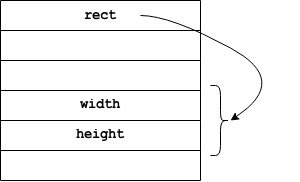
\includegraphics[width=6cm]{images/instantiatedObject.png}
%\end{center}

  \begin{itemize}
  \item These can be combined:
\begin{lstlisting}[basicstyle=\small]
ClassName classVar = new ClassName(); 
//declaration + instantiation

Rectangle r = new Rectangle(); //example
\end{lstlisting}
  \end{itemize}

\begin{exercise}[4][Declare and Instantiate an object]
Declare and instantiate an object \texttt{myCircle} of class \texttt{Circle}
\end{exercise}
\begin{answer}
\begin{lstlisting}
public class Client {
	public static void main(String[] args) {
		Circle myCircle = new Circle();
	}
}
\end{lstlisting}	
Although, you can just write the relevant part in written exams:
\begin{lstlisting}
Circle myCircle = new Circle();
\end{lstlisting}
\end{answer}

\subsection{Adding method to a class}

You can add methods inside the class that can be called on any \textit{instance} of the class.

\lstinputlisting{code/Rectangle0.5.java}

\vskip 0.1cm
\begin{center}
	\begin{tikzpicture}
		\umlclass{Rectangle}
		{
			+ width : double\\
			+ height : double\\				
		}
		{
			+ area (  ) : double\\
			+ isSquare(  ) : boolean\\		
		}
	\end{tikzpicture}				
\end{center}
\vskip 0.1cm

\subsection{The dot (.) operator}
  The dot operator gives us access to the members (instance variables and method) for an object. Think of it as the \texttt{apostrophe s ('s)} of the human language (as in \emph{"Gaurav's class"} or \emph{"Matt's workshop"})
   
  \begin{lstlisting}
  Rectangle r = new Rectangle(); //example
  r.width = 5;
  \end{lstlisting}


    \begin{itemize}
  	\item The expression \texttt{r} gives us access to the instance variable \texttt{width} of object \texttt{r}.
  
  	\item When a method is invoked on an object using the dot operator, it calls the method as defined in the class \textbf{in the context} of that object and any instance variables used in that method are the ones belonging to that object.
	\end{itemize}

    \begin{lstlisting}
  Rectangle r = new Rectangle(); 
  r.width = 5;
  r.height = 8;
  System.out.println(r.area());
  \end{lstlisting}

  \vskip 0.5cm
  
  
  Here, \texttt{r.area()} returns \texttt{width * height} and since the method is called on object \texttt{r}, it returns \texttt{r.width * r.height}. Had the method been called on another object \texttt{s}, it would return \texttt{s.width * s.height}.
  
\begin{exercise}[5][Access instance variables and call methods]
Write a piece of code that sits outside the class definition and displays the radius of the object \texttt{myCircle} and also its area.
\end{exercise}
\begin{answer} \begin{lstlisting}
System.out.println(myCircle.getRadius());
System.out.println(myCircle.area());
\end{lstlisting} \end{answer}

\subsection{Are there any default values?}

    \begin{itemize}
    \item Each {\em instance variables}	
          is automatically initialised to the default value for its type when an object of
          the class is created. 
    \item For example, an instance variable
          of type \lstinline!int! is given the default value 0;
    \item And an instance variable
          of type \lstinline!String! (or any class type)
          is given the default value \lstinline!null!.
          (More about \lstinline!null! later.)
    \end{itemize}

\section{Getters and setters}
\subsection{Bad client, bad bad client!}

Once the object is created, we can start operating on it.
\begin{lstlisting}[style=buggy]
Rectangle r = new Rectangle();
@r.width = -5;@ // :o :O
r.height = 8;
System.out.println(r.area()); 
//displays -40 :'(
\end{lstlisting}

\subsection{Changing visibility to private}

\lstinputlisting{code/Rectangle1.java}

\vskip 0.1cm
\begin{center}
		\begin{tikzpicture}
			\umlclass{Rectangle}
			{
				- width : double\\
				- height : double\\				
			}
			{
				+ area ( ) : double\\
				+ isSquare ( ) : boolean\\				
			}
		\end{tikzpicture}
\end{center}
\vskip 0.1cm

Now, the instance variables \texttt{width} and \texttt{height} are visible only within the class definition.

\subsection{How does one access (read/write) private instance variables}

We access (read and write) private instance variables through public methods called \texttt{getters} and \texttt{setters}.
\begin{itemize}
\item \texttt{getters} return the value of the instance variable to the caller.
\item \texttt{setters} set the value supplied by the caller to the instance variables.
\end{itemize}

\lstinputlisting{code/Rectangle2.java}

\subsection{Setters must provide validation where applicable}

You can see that we validated the passed values before assigning to the instance variable as
	\texttt{width = Math.abs(w)}. This is a typical case and setters are in charge of validating data before assigning it to the instance variables. 	

\vskip 0.1cm
\begin{center}
		\begin{tikzpicture}
			\umlclass{Rectangle}
			{
				- width : double\\
				- height : double\\
			}
			{
				+ getWidth ( ) : double\\
				+ getHeight ( ) : double\\			
				+ setWidth ( width : double ) : void\\
				+ setHeight ( height : double ) : void\\
				+ area ( ) : double\\
				+ perimeter ( ) : double\\		
				+ isSquare ( ) : boolean \\	
			}
		\end{tikzpicture}	
\end{center}
\vskip 0.1cm

\begin{exercise}[8][Add getters and setters]
Add getters and setters to class \texttt{Circle}. The setter should result in radius becoming zero if the parameter passed is not positive.
\end{exercise}
\begin{answer} \begin{lstlisting}
//setter
public void setRadius(double r) {
	if(r < 0)
		radius = 0;
	else
		radius = r;
}

//getter
public double getRadius() {
	return radius;
}
\end{lstlisting} \end{answer}

\begin{exercise}[6][Write a client]
Write a client (code sitting outside \texttt{Circle.java}, for example, in the \texttt{main} method of another class) that performs the following operations,

\begin{itemize}
\item Declare and instantiate object \texttt{myCircle} of class \texttt{Circle} that has a radius of 1.8
\item Display radius of \texttt{myCircle}.
\item Increase radius of \texttt{myCircle} by 1.4
\end{itemize}
\end{exercise}
\begin{answer} \begin{lstlisting}
public class Client {
	public static void main(String[] args) {
		Circle myCircle = new Circle();
		myCircle.setRadius(1.8);
		System.out.println(myCircle.getRadius());
		myCircle.setRadius(myCircle.getRadius() + 1.4);
		/* or you can split it up as:
		* double current = myCircle.getRadius();
		* double updated = current + 1.4;
		* myCircle.setRadius(updated);
		*/
	}
}
\end{lstlisting} \end{answer}

\subsection{I wish creating objects was easier}

Let's say that the user wants to create a \texttt{Rectangle} whose \texttt{width} is 5 and \texttt{height} is 8. Following code achieves this,

\begin{lstlisting}
Rectangle r = new Rectangle();
r.width = 5;
r.height = 8;
\end{lstlisting}

However, it would be really nice if one could pass the values for the instance variables in the instantiation statement itself, as,

\begin{lstlisting}
Rectangle r = new Rectangle(5, 8);
\end{lstlisting}

This is done through \texttt{constructors}.

\section{Constructors}
\begin{itemize}
\item A constructor is a method defined in the class.
\item A constructor must have the same name as the class.
\item A constructor has no return type (not even void).
\item There may be multiple constructors, each distinguished by its parameter list. Thus, we may have one constructor with no parameters, and another with one \texttt{int} parameter.
\item A suitable constructor is automatically called during instantiation based on number of parameters passed. If an appropriate constructor is not found, a compilation error is generated.
\end{itemize}

\subsection{Example - Constructor}

\begin{lstlisting}[basicstyle=\tiny]
public class Rectangle {
    private double width, height;
    
    //getters and setters

    public Rectangle() { //default constructor
		setWidth(1);
		setHeight(1);
    }

    //parameterized constructor for a square
    public Rectangle(double side) { 
		setWidth(side);
		setHeight(side);
    }

    //parameterized constructor - generic
    public Rectangle(double w, double h) { 
		setWidth(w);
		setHeight(h);
    }
    //rest of the code
}
\end{lstlisting}

\vskip 0.1cm
\begin{center}
		\begin{tikzpicture}
			\umlclass{Rectangle}
			{
				- width : double\\
				- height : double\\
			}
			{
				+ getWidth ( ) : double\\
				+ getHeight ( ) : double\\			
				+ setWidth ( width : double ) : void\\
				+ setHeight ( height : double ) : void\\
				+ Rectangle ( )\\
				+ Rectangle ( side : double )\\
				+ Rectangle ( w : double, h : double )\\
				+ area ( ) : double\\
				+ perimeter ( ) : double\\	
				+ isSquare( ) : boolean\\		
			}
		\end{tikzpicture}
\end{center}
\vskip 0.1cm

\subsection{Constructors should call setters - always!}

\textbf{Constructors should \color{red}always \color{black} use setters to assign values to instance variables.}

\subsection{Default constructor}

It should be noted that a default constructor (without any parameters) is pre-defined for you by Java and that's why you can instantiate objects without defining it yourself.

\begin{lstlisting}
Rectange r = new Rectangle();
\end{lstlisting}

The default constructor assigns the default values for the appropriate data types to the instance variables. However, once you define a parameterized constructor, the built-in default constructor is taken away by Java. Thus, if you want to construct an object with default initial values for the instance variables, you need to re-define that!


\subsection{Defining the default constructor}

Let's say the default \texttt{Rectangle} instance should be of unit length. We can define the default constructor as,
\begin{lstlisting}
public Rectangle() {
	setLength(1);
	setBreadth(1);
}
\end{lstlisting}

\begin{exercise}[8][Add default and parameterized constructor]
Add two constructors to the class \texttt{Circle}.
\begin{enumerate}
\item No parameters passed (default constructor): Assigns the value 1.0 to radius ... through the setter.
\item Parameter passed for radius (parameterized constructor): Assigns the passed value to radius through the setter.
\end{enumerate}
\end{exercise}
\begin{answer} \begin{lstlisting}
//default constructor
public Circle() {
	setRadius(1);
}

//parameterized constructor
public Circle(double r) {
	setRadius(r); //let setter handle the validation
}
\end{lstlisting} \end{answer}


\section{Displaying objects}

Often we need to display the details of an object. For example, we might need to display name and age of a Person object, or the details of a Time object in the format \texttt{hours:minutes:seconds}, or in our example, \texttt{width} and \texttt{height} of a \texttt{Rectangle} object. It is quite inconvenient to display these details as,

\begin{lstlisting}
Rectangle r = new Rectangle(5, 8);
System.out.println(r.width+`` by ''+r.height);
\end{lstlisting}

We \emph{could} add a method \texttt{display} in the class \texttt{Rectangle} as,

\begin{lstlisting}
public void display() {
    System.out.println(width+`` by ''+height);
}
\end{lstlisting}

And call this method on required object as,

\begin{lstlisting}
Rectangle r = new Rectangle(5, 8);
r.display();
\end{lstlisting}

\subsection{Problem with the \texttt{display()} method}

But this would only let us \textbf{display} the object details, and not send to a file, or concatenate with any other output. 

Java provides a standard way to return the String description of an object using the \texttt{toString()} method (with return type \texttt{String}). 

\subsection{Default \texttt{toString()} behaviour}

When you display an object, what Java displays is the outcome of the {toString()} method on that object
\begin{lstlisting}
Rectangle r = new Rectangle(1, 3);
System.out.println(r); //something like [I@70dea4e
\end{lstlisting}

Java saw that you want to display a \texttt{Rectangle} object and replaced it by the \texttt{toString()} method operating on that object as,

\begin{lstlisting}
System.out.println(r);
//became
System.out.println(r.toString()); 
\end{lstlisting}

\subsection{Over-riding \texttt{toString()} behaviour}

We can over-ride \texttt{toString()} method as required. For the \texttt{Rectangle} class,

\begin{lstlisting}
public String toString() {
    return width+`` by ''+height;
}
\end{lstlisting}

When we display an object, it invokes the method \texttt{toString()} and displays the value it returns.

\begin{lstlisting}
Rectangle r = new Rectangle(5, 8);
System.out.println(r);
/*
automatically invokes r.toString() 
and displays the value returned
*/
\end{lstlisting}

\begin{exercise}[5][Define toString method]
Define the \texttt{toString} method in the \texttt{Circle} class such that it displays the object details in the following format -

\begin{verbatim}
Circle radius: <radius>, area: <area>
\end{verbatim}

In a separate client, create a Circle object with radius 1.6 and display it on the console.
\end{exercise}
\begin{answer} \begin{lstlisting}
public String toString() {
	String result = "Circle radius: "+radius+", area: "+area();
	return result;
}	
\end{lstlisting} \end{answer}

\section{Class containing an array}

In this unit, we'll extensively see classes containing arrays. 

We must remember that both arrays and objects are references and refer to the memory holding the actual data (in the case of array, it's the array items, and in the case of objects, it's the instance variables).

Take the following as an example (instance variables are \texttt{public} for simplicity),

\begin{lstlisting}
public class DynamicArray {
	public int[] data;
	public int nItems;
}
\end{lstlisting}

The client is as follows,

\begin{lstlisting}
public class Client {
	public static void main(String[] args) {
		DynamicArray list = new DynamicArray();
	}
}
\end{lstlisting}

At this stage, the memory state looks like,

\vskip 0.5cm

		

\newpage

If we change the values of the instance variables as,

\begin{lstlisting}
public class Client {
	public static void main(String[] args) {
		DynamicArray list = new DynamicArray();
		list.data = new int[4];
		list.nItems = 0;
	}
}
\end{lstlisting}

It now becomes,

\vskip 0.5cm

\begin{tikzpicture}[scale=.5]
\memoryblock{textsize=\Large,x=0,y=8.5,width=4,height=3,array={"list"}}
\memoryblock{textsize=\Large,x=8, y=6, width=8, height=5,array={"data","nItems=0"}}
\arrow{startX=3.5, startY=10, endX=8, endY=10}
\memoryblock{textsize=\Large,x=20,y=5,width=6,height=8,array={"[0]=0","[1]=0","[2]=0","[3]=0"}}
\arrow{startX=13.5, startY=10, endX=20, endY=12}
\end{tikzpicture}
\vskip 0.5cm

Finally, we can modify the items of the array as,

\begin{lstlisting}
public class Client {
	public static void main(String[] args) {
		DynamicArray list = new DynamicArray();
		list.data = new int[4];
		list.data[0] = 5;
		list.data[1] = 12;
		list.nItems = 2;
	}
}
\end{lstlisting}

\newpage
This gives us,
\vskip 0.5cm
\begin{tikzpicture}[scale=.5]
\memoryblock{textsize=\Large,x=0,y=8.5,width=4,height=3,array={"list"}}
\memoryblock{textsize=\Large,x=8, y=6, width=8, height=5,array={"data","nItems=2"}}
\arrow{startX=3.5, startY=10, endX=8, endY=10}
\memoryblock{textsize=\Large,x=20,y=5,width=6,height=8,array={"[0]=5","[1]=12","[2]=0","[3]=0"}}
\arrow{startX=13.5, startY=10, endX=20, endY=12}
\end{tikzpicture}
\input{comp125lectureFooter}